\documentclass[14pt]{extbook}
\usepackage{multicol, enumerate, enumitem, hyperref, color, soul, setspace, parskip, fancyhdr} %General Packages
\usepackage{amssymb, amsthm, amsmath, bbm, latexsym, units, mathtools} %Math Packages
\everymath{\displaystyle} %All math in Display Style
% Packages with additional options
\usepackage[headsep=0.5cm,headheight=12pt, left=1 in,right= 1 in,top= 1 in,bottom= 1 in]{geometry}
\usepackage[usenames,dvipsnames]{xcolor}
\usepackage{dashrule}  % Package to use the command below to create lines between items
\newcommand{\litem}[1]{\item#1\hspace*{-1cm}\rule{\textwidth}{0.4pt}}
\pagestyle{fancy}
\lhead{Makeup Progress Quiz 1}
\chead{}
\rhead{Version A}
\lfoot{6018-3080}
\cfoot{}
\rfoot{Spring 2021}
\begin{document}

\begin{enumerate}
\litem{
Determine the domain of the function below.\[ f(x) = \frac{6}{9x^{2} +3 x -20} \]\begin{enumerate}[label=\Alph*.]
\item \( \text{All Real numbers except } x = a \text{ and } x = b, \text{ where } a \in [-16, -14] \text{ and } b \in [12, 14] \)
\item \( \text{All Real numbers except } x = a \text{ and } x = b, \text{ where } a \in [-3.67, 0.33] \text{ and } b \in [1.33, 5.33] \)
\item \( \text{All Real numbers.} \)
\item \( \text{All Real numbers except } x = a, \text{ where } a \in [-16, -14] \)
\item \( \text{All Real numbers except } x = a, \text{ where } a \in [-3.67, 0.33] \)

\end{enumerate} }
\litem{
Solve the rational equation below. Then, choose the interval(s) that the solution(s) belongs to.\[ \frac{-2x}{-7x + 6} + \frac{-6x^{2}}{28x^{2} +25 x -42} = \frac{-4}{-4x -7} \]\begin{enumerate}[label=\Alph*.]
\item \( x \in [3.5,7.7] \)
\item \( x_1 \in [2.5, 3.8] \text{ and } x_2 \in [-1.14,3.86] \)
\item \( \text{All solutions lead to invalid or complex values in the equation.} \)
\item \( x \in [-4.1,0.9] \)
\item \( x_1 \in [2.5, 3.8] \text{ and } x_2 \in [2,9] \)

\end{enumerate} }
\litem{
Choose the graph of the equation below.\[ f(x) = \frac{-1}{(x + 3)^2} + 1 \]\begin{enumerate}[label=\Alph*.]
\begin{multicols}{2}\item 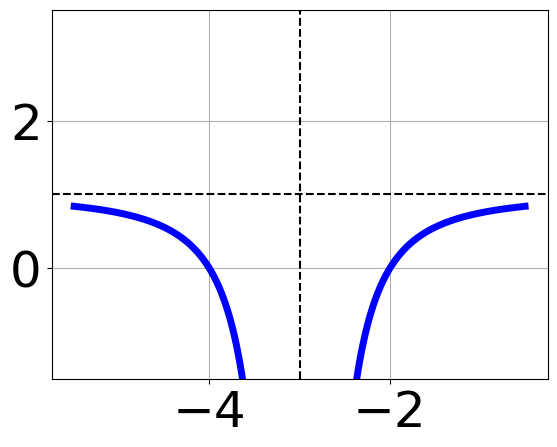
\includegraphics[width = 0.3\textwidth]{../Figures/rationalEquationToGraphCopyAA.png}\item 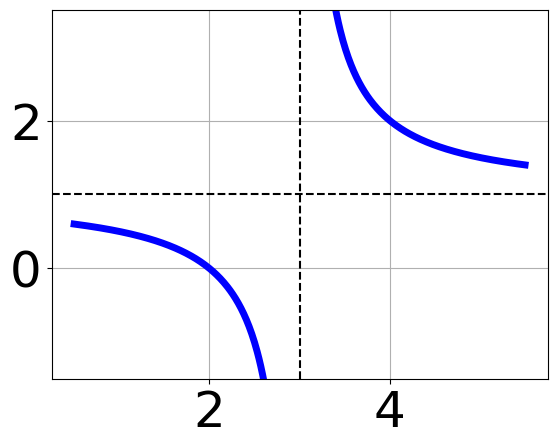
\includegraphics[width = 0.3\textwidth]{../Figures/rationalEquationToGraphCopyBA.png}\item 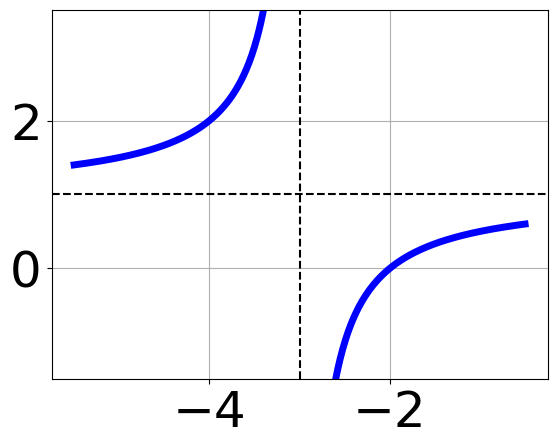
\includegraphics[width = 0.3\textwidth]{../Figures/rationalEquationToGraphCopyCA.png}\item 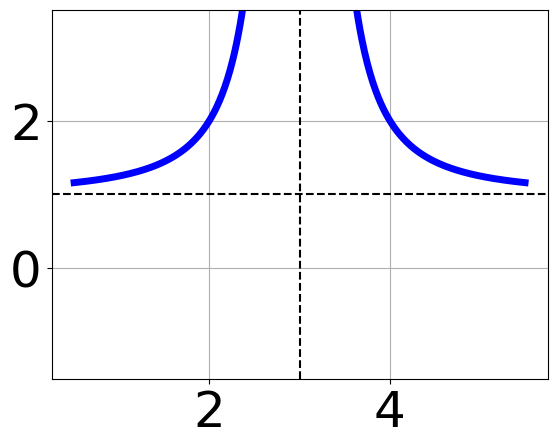
\includegraphics[width = 0.3\textwidth]{../Figures/rationalEquationToGraphCopyDA.png}\end{multicols}\item None of the above.
\end{enumerate} }
\litem{
Choose the graph of the equation below.\[ f(x) = \frac{1}{x + 3} - 2 \]\begin{enumerate}[label=\Alph*.]
\begin{multicols}{2}\item 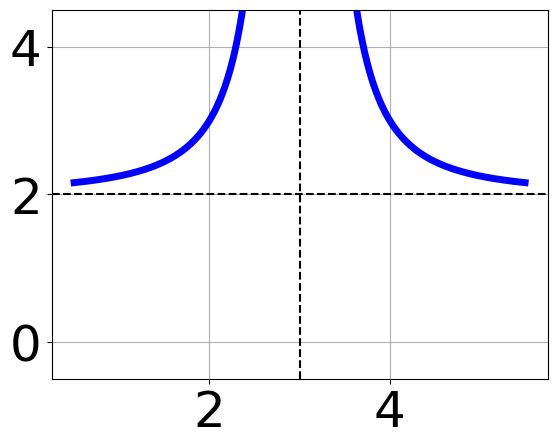
\includegraphics[width = 0.3\textwidth]{../Figures/rationalEquationToGraphAA.png}\item 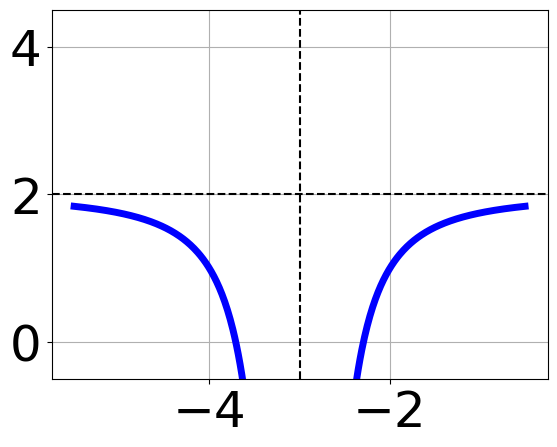
\includegraphics[width = 0.3\textwidth]{../Figures/rationalEquationToGraphBA.png}\item 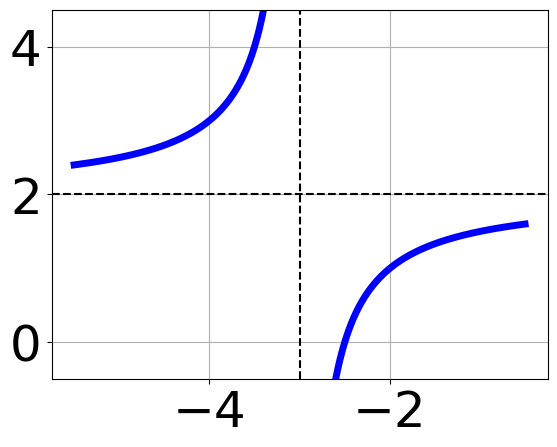
\includegraphics[width = 0.3\textwidth]{../Figures/rationalEquationToGraphCA.png}\item 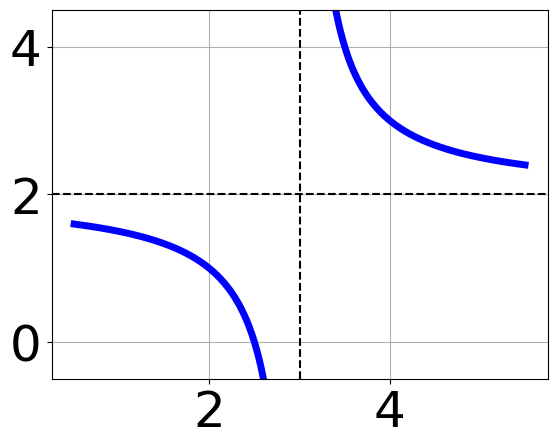
\includegraphics[width = 0.3\textwidth]{../Figures/rationalEquationToGraphDA.png}\end{multicols}\item None of the above.
\end{enumerate} }
\litem{
Choose the equation of the function graphed below.
\begin{center}
    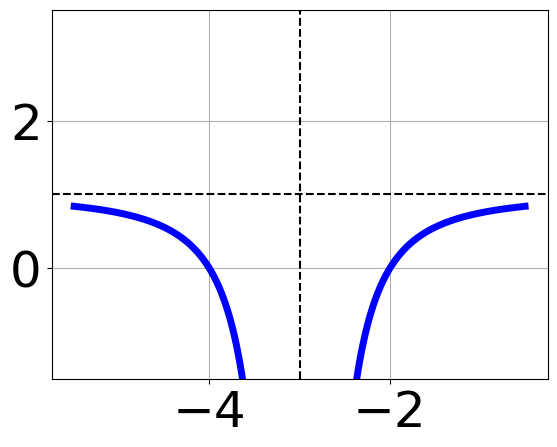
\includegraphics[width=0.5\textwidth]{../Figures/rationalGraphToEquationCopyA.png}
\end{center}
\begin{enumerate}[label=\Alph*.]
\item \( f(x) = \frac{1}{(x + 3)^2} - 2 \)
\item \( f(x) = \frac{1}{x + 3} - 2 \)
\item \( f(x) = \frac{-1}{x - 3} - 2 \)
\item \( f(x) = \frac{-1}{(x - 3)^2} - 2 \)
\item \( \text{None of the above} \)

\end{enumerate} }
\litem{
Solve the rational equation below. Then, choose the interval(s) that the solution(s) belongs to.\[ \frac{-4x}{3x + 7} + \frac{-6x^{2}}{-15x^{2} -23 x + 28} = \frac{6}{-5x + 4} \]\begin{enumerate}[label=\Alph*.]
\item \( x_1 \in [-5.8, 0.2] \text{ and } x_2 \in [-5.33,0.67] \)
\item \( x \in [1.7,6.1] \)
\item \( x \in [-0.1,2.2] \)
\item \( \text{All solutions lead to invalid or complex values in the equation.} \)
\item \( x_1 \in [-5.8, 0.2] \text{ and } x_2 \in [2.33,12.33] \)

\end{enumerate} }
\litem{
Determine the domain of the function below.\[ f(x) = \frac{5}{36x^{2} +54 x + 18} \]\begin{enumerate}[label=\Alph*.]
\item \( \text{All Real numbers except } x = a, \text{ where } a \in [-36.22, -34.75] \)
\item \( \text{All Real numbers except } x = a, \text{ where } a \in [-2.17, -0.85] \)
\item \( \text{All Real numbers.} \)
\item \( \text{All Real numbers except } x = a \text{ and } x = b, \text{ where } a \in [-36.22, -34.75] \text{ and } b \in [-18.97, -17.51] \)
\item \( \text{All Real numbers except } x = a \text{ and } x = b, \text{ where } a \in [-2.17, -0.85] \text{ and } b \in [-0.79, -0.36] \)

\end{enumerate} }
\litem{
Choose the equation of the function graphed below.
\begin{center}
    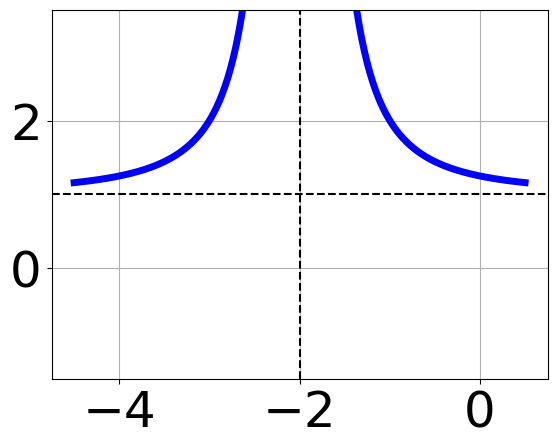
\includegraphics[width=0.5\textwidth]{../Figures/rationalGraphToEquationA.png}
\end{center}
\begin{enumerate}[label=\Alph*.]
\item \( f(x) = \frac{1}{(x - 2)^2} + 1 \)
\item \( f(x) = \frac{1}{x - 2} + 1 \)
\item \( f(x) = \frac{-1}{(x + 2)^2} + 1 \)
\item \( f(x) = \frac{-1}{x + 2} + 1 \)
\item \( \text{None of the above} \)

\end{enumerate} }
\litem{
Solve the rational equation below. Then, choose the interval(s) that the solution(s) belongs to.\[ \frac{-6}{-4x -9} + 6 = \frac{5}{20x + 45} \]\begin{enumerate}[label=\Alph*.]
\item \( x \in [0.9,4.1] \)
\item \( x \in [-3.46,-1.46] \)
\item \( x_1 \in [-4.1, -2.7] \text{ and } x_2 \in [-2.46,-0.46] \)
\item \( x_1 \in [-2.6, -2.4] \text{ and } x_2 \in [0.04,3.04] \)
\item \( \text{All solutions lead to invalid or complex values in the equation.} \)

\end{enumerate} }
\litem{
Solve the rational equation below. Then, choose the interval(s) that the solution(s) belongs to.\[ \frac{3}{-4x + 8} + -2 = \frac{-4}{-32x + 64} \]\begin{enumerate}[label=\Alph*.]
\item \( x \in [1.56,2.56] \)
\item \( x_1 \in [0.5, 1.31] \text{ and } x_2 \in [1.56,3.56] \)
\item \( x_1 \in [-2.7, -1.89] \text{ and } x_2 \in [1.56,3.56] \)
\item \( x \in [-2.7,-1.89] \)
\item \( \text{All solutions lead to invalid or complex values in the equation.} \)

\end{enumerate} }
\end{enumerate}

\end{document}